% Provenance (never printed): see sources/outline_sources.md (Year 3: the
% structure of the Galaxy; the rotation curve and dark matter; galaxy types;
% the distance ladder, Hubble's law recalled from the physics books).
% Brief: sources/book5/BRIEFS.md, ch. 29. Curves from figdata/bachelor-3/
% rotation_curve.py (the circular velocity curve of Eilers et al. 2019 with the
% Pouliasis et al. 2017 Model I baryons and an NFW halo fitted to it) and
% distance_ladder.py (the OGLE-IV Cepheids of the Large Magellanic Cloud, CDS
% J/AcA/65/297, and the ranges of the rungs). Exercise and problem values in the
% Book 5 scratch calculator calc/ch29.py. The survey of Part I of the problem and
% the galaxies of the exercises are invented.
\chapter{درب التبانة والمجرّات}\label{ch:b3:milky-way-galaxies}

في المجموعة الشمسية تتحرّك الكواكب البعيدة عن الشمس ببطء: يدور عطارد
حولها بسرعة \qty{47.4}{km.s^{-1}}، ونبتون بسرعة \qty{5.4}{km.s^{-1}}، كما يقتضي
قانون كبلر الثالث للأجسام المرتبطة بكتلة مركزية واحدة. أمّا نجوم
درب التبانة فلا تسلك هذا السلوك. ويُقاس من حركات أكثر من
عشرين ألف عملاق أحمر، وتبلغ سرعة مداراتها الدائرية
\qty{227}{km.s^{-1}} على بعد \qty{5}{kpc} من المركز، و\qty{229}{km.s^{-1}}
عند الشمس، ولا تزال \qty{198}{km.s^{-1}} عند \qty{25}{kpc}، حيث يكاد لا يبقى
أيّ نجوم أو غاز. ولو كانت الكتلة المرئية هي كلّ ما هناك، لكانت النجوم الخارجية
أبطأ بكثير. ثمّة شيء غير مرئي يُمسكها. يصف هذا الفصل درب التبانة التي نعيش فيها،
ويزنها من دورانها، ويصنّف المجرّات الأخرى إلى أنماط،
ويصعد سلسلة الطرائق التي تُقاس بها مسافاتها،
وكذلك توسّع الكون.
% ledger: planet:Mercury.vorb, planet:Neptune.vorb, eilers19:vc, eilers19:table1

\begin{recall}
درب التبانة، وتأثير دوبلر، وقوانين كبلر، ومبرهنة نيوتن عن جذب القشرة الكروية،
والمادة المظلمة، والثقب الأسود ونصف قطر شوارتزشيلد له، والمستعرات الأعظم،
والأقزام البيضاء، وخطّ 21 سم للهيدروجين الذرّي، وقانون هابل
ترد في كتب الفيزياء. أمّا الاختلاف المنظري السنوي والفرسخ الفلكي
والدفق والإشعاعية، والقدر الظاهري والمطلق، ومعامل المسافة، والنطاقات الضوئية
ودليل اللون، فترد في
مجلد السنة الأولى، في فصله عن التلسكوبات والقياس الضوئي. أمّا الوسط بين النجمي
وغباره فترد في مجلد السنة الثانية، في فصله عن الوسط بين النجمي
وتكوّن النجوم.
\end{recall}

\section{بنية درب التبانة}\label{sec:b3:milky-way-galaxies:structure}

عند النظر من الأرض، يبدو درب التبانة حزامًا من الضوء يحيط بالسماء
كلّها، تقطعه ممرّات معتمة من الغبار، وأشدّ ما يكون سطوعًا نحو
كوكبة القوس حيث يقع مركزه. والحزام هو القرص الذي تقع فيه الشمس،
ويُرى من داخله على حافّته.

\begin{omfigure}
\centering
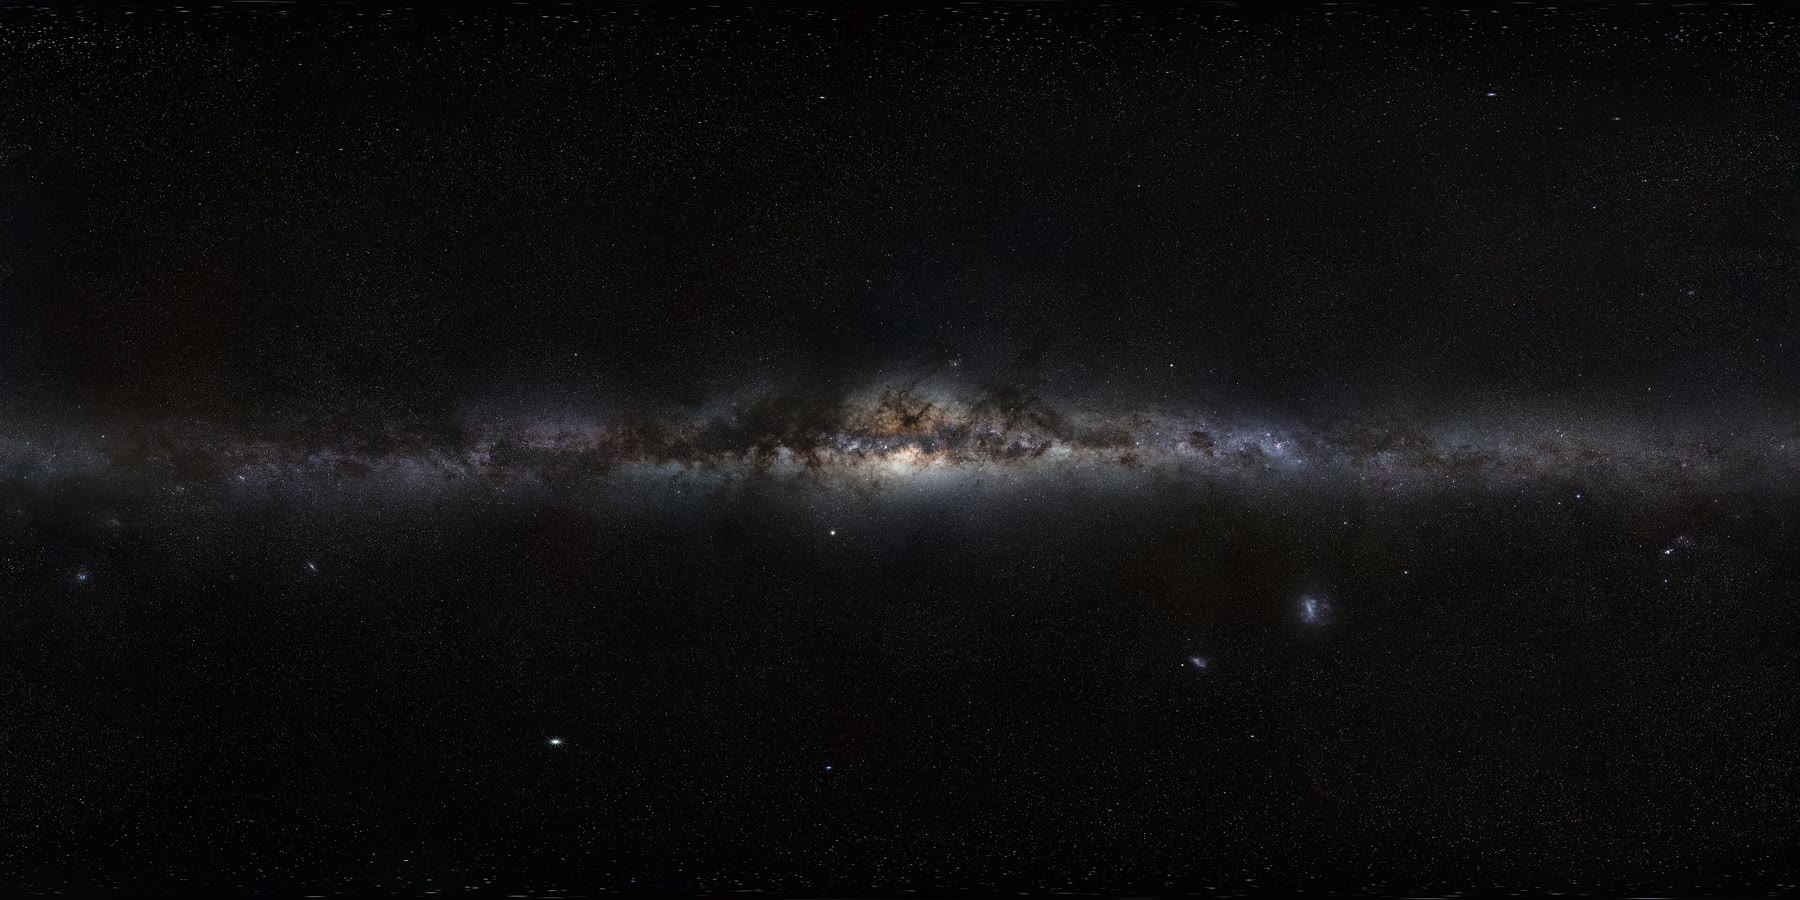
\includegraphics[width=0.96\linewidth]{images/book5/b3-milky-way-panorama.jpg}
\par\smallskip{\small السماء كلّها في صورة واحدة، مُسقطةً بحيث
يمتدّ مستوى درب التبانة عبر وسط الصورة ويقع مركزه عند
مركز الصورة. والحزام هو القرص المرئي من داخله، والممرّات المعتمة
هي غبار في القرص يحجب النجوم خلفه، والانتفاخ المركزي
ينتفخ حول المركز. والبقعتان الصغيرتان أسفل الحزام، إلى
اليمين، هما سحابتا ماجلان الكبرى والصغرى، وهما مجرّتان تابعتان؛
والبقعة الباهتة أسفل الحزام قرب الحافّة اليسرى هي مجرّة
أندروميدا. الصورة: \mbox{\textdir TLT ESO/S.~Brunier, CC BY~4.0}.}\label{fig:b3:milky-way-galaxies:panorama}
\end{omfigure}
% ledger: photo:b3-milky-way-panorama, mcconn12:local-group

\begin{definition}[القرص المجرّي، والقرص السميك، والانتفاخ المجرّي والهالة النجمية]\label{def:b3:milky-way-galaxies:structure}
\emph{القرص المجرّي}\index{القرص المجرّي} هو المكوّن المفلطح من درب
التبانة، ويتألّف من نجوم وغاز وغبار في مدارات شبه دائرية حول مركزه؛
تتناقص كثافته تقريبًا تناقصًا أُسّيًّا مع الارتفاع فوق مستواه المتوسّط
ومع البعد عن مركزه، ويُعبَّر عن ذلك بالارتفاع المميّز والطول
المميّز. \emph{القرص السميك}\index{القرص السميك} مكوّن قرصي ثانٍ أقدم،
ذو ارتفاع مميّز أكبر وكتلة أصغر. أمّا
\emph{الانتفاخ المجرّي}\index{الانتفاخ المجرّي} هو التجمّع المركزي
للنجوم الذي ينتفخ خارج القرص. أمّا \emph{الهالة النجمية}\index{الهالة النجمية}
فهي المكوّن المتفرّق شبه الكروي من النجوم القديمة والعناقيد الكروية
التي تحيط بالقرص والانتفاخ.
\end{definition}

درب التبانة مجرّة حلزونية ذات قضيب. وفي جوار الشمس يبلغ الارتفاع المميّز للقرص الرقيق
نحو \qty{300}{pc}، وللقرص السميك
\qty{900}{pc}؛ وتبلغ أطوالها المميّزة نحو \qty{2.6}{kpc}
و\qty{2.0}{kpc}. يحتوي \omterm{def:b3:milky-way-galaxies:structure}{القرص السميك} على نحو \num{6e9} كتلة شمسية،
نحو خُمس كتلة القرص الرقيق. ويبدو الانتفاخ من الجانب كصندوق
أو كالفول السوداني، وهو الجزء الداخلي المنتفخ من قضيب نجمي يبلغ نصف طوله نحو
\qty{5}{kpc}، ويصنع محوره الطويل زاوية قدرها
\ang{27} مع الخطّ الواصل من الشمس إلى المركز. وتضمّ \omterm{def:b3:milky-way-galaxies:structure}{الهالة النجمية}
نحو واحد في المئة فقط من النجوم. وفي المجموع تزن نجوم درب التبانة نحو
\num{5e10} كتلة شمسية.
% ledger: bhg16:structure

\begin{omfigure}
\centering
\begin{tikzpicture}[x=0.17cm, y=0.17cm, font=\scriptsize]
% edge-on view
\begin{scope}
\fill[omProp!8] (0,0) circle (17);
\draw[omProp!60, densely dotted] (0,0) circle (17);
\fill[black!12] (0,0) ellipse (15 and 2.4);
\fill[black!30] (0,0) ellipse (15 and 0.8);
\fill[black!45] (-3.2,0) .. controls (-3.4,2.3) and (-1.2,2.0) .. (0,1.4)
  .. controls (1.2,2.0) and (3.4,2.3) .. (3.2,0)
  .. controls (3.4,-2.3) and (1.2,-2.0) .. (0,-1.4)
  .. controls (-1.2,-2.0) and (-3.4,-2.3) .. (-3.2,0) -- cycle;
\foreach \p in {(-10,9),(6,12),(12,-7),(-6,-13),(-13,-4),(3,-9),(12,8)}
  \fill[omProp] \p circle (0.35);
\fill[ocYellow, draw=black] (-8.2,0.15) circle (0.55);
\node[anchor=south] at (-8.2,0.9) {الشمس};
\draw[|<->|] (0,-4.6) -- node[below] {$R_0 \approx \qty{8.2}{kpc}$} (-8.2,-4.6);
\node[anchor=west] at (15.3,0) {القرص الرقيق};
\node[anchor=west] at (13.2,2.8) {القرص السميك};
\draw[->] (4.6,4.6) node[anchor=south west, inner sep=1pt] {الانتفاخ} -- (2.4,1.7);
\node[omProp!80!black] at (-11,13.5) {الهالة النجمية};
\node at (0,-19.5) {\foreignlanguage{arabic}{(أ) منظورًا من الحافّة}};
\end{scope}
% face-on view
\begin{scope}[xshift=7.6cm]
\fill[omProp!8] (0,0) circle (17);
\draw[omProp!60, densely dotted] (0,0) circle (17);
\fill[black!12] (0,0) circle (15);
\foreach \a in {0,180} {
  \draw[line width=1.6pt, black!40, rotate=\a+63]
    plot[domain=0:3.9, samples=50] ({5*exp(0.25*\x)*cos(\x r)}, {5*exp(0.25*\x)*sin(\x r)});
}
\fill[black!45, rotate=63] (0,0) ellipse (5 and 1.5);
\draw[dashed] (0,0) circle (8.2);
\fill[ocYellow, draw=black] (0,-8.2) circle (0.55);
\node[anchor=north] at (0,-8.9) {الشمس};
\draw[dotted, thick] (0,0) -- (0,-8.2);
\draw[thick, ->] (0,0) ++(25:16) arc (25:-25:16);
\node[anchor=west] at (17.3,0) {الدوران};
\node[anchor=west, fill=black!12, inner sep=1pt] at (3.4,3.4) {القضيب};
\draw[|-|] (6,-15.5) -- node[below] {\qty{5}{kpc}} (11,-15.5);
\node at (0,-19.5) {\foreignlanguage{arabic}{(ب) منظورًا من القطب المجرّي الشمالي}};
\end{scope}
\end{tikzpicture}
\par\smallskip{\small رسم تخطيطي لدرب التبانة بالمقياس الصحيح لأبعادها
الرئيسية. (أ)~منظورًا من الحافّة: القرص الرقيق (النطاق الداكن)، \omterm{def:b3:milky-way-galaxies:structure}{والقرص السميك} (النطاق
الفاتح)، والانتفاخ ذو الهيئة الصندوقية، \omterm{def:b3:milky-way-galaxies:structure}{والهالة النجمية} مع عناقيدها الكروية
(النقاط البرتقالية)؛ وتقع الشمس في القرص على بعد نحو \qty{8.2}{kpc}
من المركز، وعلى ارتفاع نحو \qty{25}{pc} فوق المستوى المتوسّط (أصغر من أن
يظهر). (ب)~منظورًا من القطب المجرّي الشمالي: القضيب، ويبلغ نصف طوله نحو
\qty{5}{kpc}، ومائل بزاوية \ang{27} عن الخطّ الواصل من الشمس
إلى المركز (منقّطًا)؛ والدائرة الشمسية (متقطّعة)؛ والأذرع \omterm{def:b3:milky-way-galaxies:types}{الحلزونية} مرسومة
تخطيطيًّا؛ وتدور درب التبانة في اتجاه عقارب الساعة في هذا المنظور.}\label{fig:b3:milky-way-galaxies:sketch}
\end{omfigure}
% ledger: bhg16:structure, gravity19:r0

\begin{definition}[الجمهرة النجمية]\label{def:b3:milky-way-galaxies:populations}
\emph{الجمهرة النجمية}\index{الجمهرة النجمية} هي مجموعة من النجوم
في مجرّة ما تتشارك مدًى من الأعمار والتراكيب الكيميائية
والمدارات. النجوم الفتيّة في القرص الرقيق، الغنيّة بعناصر أثقل من
الهيليوم والواقعة في مدارات شبه دائرية، يُطلق عليها تقليديًّا
الجمهرة~I؛ أمّا النجوم القديمة في الهالة وفي العناقيد الكروية، الفقيرة
في العناصر الثقيلة والواقعة في مدارات ذات حركات عشوائية كبيرة مع
دوران صافٍ ضئيل، فتُعرف بالجمهرة~II.
\end{definition}

يقع \omterm{def:b3:milky-way-galaxies:structure}{القرص السميك} بين الاثنين: نجومه أقدم في الغالب من نجوم
القرص الرقيق، وهي عند محتوى حديد معيّن أغنى بالعناصر الخفيفة
التي يسمّيها الفلكيون عناصر ألفا، مقيسةً نسبةً إلى الحديد. \omterm{def:b3:milky-way-galaxies:structure}{والهالة
النجمية} هي
سجلّ أحفوريّ: جرى تجميع معظمها من مجرّات صغيرة سقطت
في المجرّة ومزّقتها قوى مدّها، ولا يزال بعض تيّاراتها من النجوم
ممكنةَ التتبّع عبر السماء.
% ledger: bhg16:populations

\begin{definition}[الإحداثيات المجرّية]\label{def:b3:milky-way-galaxies:coordinates}
\emph{الإحداثيات المجرّية}\index{الإحداثيات المجرّية} لاتجاهٍ ما
هي \emph{خط العرض المجرّي} $b$، أي الزاوية المقيسة من المستوى المجرّي
(موجبة نحو القطب المجرّي الشمالي)، و\emph{خط الطول
المجرّي} $\ell$، ويُقاس في المستوى من اتجاه مركز المجرّة
($\ell = 0$) عبر $\ell = \ang{90}$، وهو
الاتجاه الذي يحمل دوران المجرّة الشمسَ نحوه. عُرّف المستوى في عام 1958
بوصفه المستوى الرئيسي للهيدروجين الذرّي في المجرّة؛
ويقع القطب المجرّي الشمالي عند المطلع المستقيم \ang{192.25}
($12^\mathrm{h}49^\mathrm{m}$) والانحراف المغناطيسي \ang{27.4} (في الاعتدال
1950).
\end{definition}
% ledger: liu11:galactic, reid20:sgra

لا تقع الشمس تمامًا في المستوى، بل تبعد نحو \qty{25}{pc} شمالَه.
وكانت مسافتها من المركز، $R_0$، لوقتٍ طويل أكثرَ الأعداد غموضًا في
علم الفلك المجرّي. وتُقاس الآن هندسيًّا: إذ يدور النجم S2 حول
الثقب الأسود المركزي للمجرّة في مدار مدّته \num{16} سنة، الذي
يعطي حجمُه الزاوي على السماء وسرعتُه على خط النظر، المرصودان
خلال 27 سنة، المسافةَ إلى المركز مباشرةً:
$R_0 = \qty{8178}{pc}$، بخطأ إحصائي مقداره \qty{13}{pc} وخطأ
منهجي مقداره \qty{22}{pc}. وتعطي مراجعةٌ لجميع الطرائق:
$R_0 = \qty[separate-uncertainty=true]{8.2 \pm 0.1}{kpc}$.
% ledger: bhg16:structure, gravity19:r0

\section{الدوران والهالة المظلمة}\label{sec:b3:milky-way-galaxies:rotation}

\begin{definition}[معيار السكون المحلي]\label{def:b3:milky-way-galaxies:lsr}
\emph{معيار السكون المحلي}\index{معيار السكون المحلي} \babelsublr{(LSR)} هو
الإطار المرجعي الذي يتحرّك على المدار الدائري حول مركز المجرّة
المارّ بالموضع الحالي للشمس. وتُقاس سرعات النجوم والغاز القريبة
منسوبةً إليه.
\end{definition}

تتحرّك الشمس بالنسبة إلى \omterm{def:b3:milky-way-galaxies:lsr}{معيار السكون المحلي} بمقدار نحو \qty{10}{km.s^{-1}} باتجاه
مركز المجرّة، و\qty{11}{km.s^{-1}} في اتجاه الدوران،
و\qty{7}{km.s^{-1}} باتجاه القطب المجرّي الشمالي: حركةٌ خاصّة صغيرة
تُضاف إلى مدار بسرعة $V_0$ تبلغ بضع مئات من الكيلومترات
في الثانية. وعند رصده من الأرض، المصدر الراديوي عند مركز
المجرّة ينجرف على امتداد المستوى المجرّي بمقدار \qty{6.411}{mas} في السنة؛ وتقريبًا
كلُّ هذا الانجراف انعكاسٌ لمدار الشمس، ومنه تُستخرج السرعة
الكلّية للشمس حول المركز، \qty[separate-uncertainty=true]{248 \pm 3}{km.s^{-1}}
(انظر \cref{exo:b3:milky-way-galaxies:2}).
% ledger: bhg16:lsr, reid20:sgra

\begin{definition}[منحنى الدوران؛ ثابتا أورت]\label{def:b3:milky-way-galaxies:rotation-curve}
\emph{منحنى الدوران}\index{منحنى الدوران} لمجرّة قرصية هو
السرعة $V(R)$ لمدار دائري في مستويها بوصفها دالّةً للبُعد
$R$ عن مركزها. وبالنسبة إلى المجرّة، مع $V_0 = V(R_0)$
و$V'_0 = \mathrm{d}V/\mathrm{d}R$ عند $R_0$، فإنّ \emph{ثابتا
أورت}\index{ثابتا أورت} هما
\[
A = \frac12\left(\frac{V_0}{R_0} - V'_0\right), \qquad
B = -\frac12\left(\frac{V_0}{R_0} + V'_0\right).
\]
\end{definition}

يقيس $A$ قصّ دوران القرص، و$B$ دوّاميّته: في
قرصٍ يدور كجسم صلب $V'_0 = V_0/R_0$ و$A = 0$؛ وعلى منحنى دوران مسطّح
$A = -B$. ويمثّل فرقُهما السرعةَ الزاوية \omterm{def:b3:milky-way-galaxies:lsr}{لمعيار السكون المحلي}،
$A - B = V_0/R_0 = \omega_0$، ويمثّل مجموعهما الميلَ $A + B = -V'_0$.

\begin{theorem}[صيغ أورت]\label{thm:b3:milky-way-galaxies:oort}
نجمٌ على بُعد $d \ll R_0$ من الشمس، في المستوى المجرّي عند
خط الطول $\ell$، على مدار دائري، له بالنسبة إلى \omterm{def:b3:milky-way-galaxies:lsr}{معيار السكون المحلي} السرعةَ الشعاعية
$v_r$ والسرعةَ المستعرضة $v_t$ (موجبة في
اتجاه تزايد $\ell$)
\[
v_r = A\,d\sin 2\ell, \qquad v_t = d\,(A\cos 2\ell + B),
\]
إلى الرتبة الأولى في $d/R_0$.
\end{theorem}

\begin{proof}
لنفرض أنّ $\omega(R) = V(R)/R$ هي السرعة الزاوية للمدار عند $R$. نضع
مركز المجرّة في نقطة الأصل، والشمس على بُعد $R_0$، وليكن
النجم على بُعد $R$ من المركز، وموضعه مرئيًّا من
المركز مُشكِّلًا الزاويةَ $\theta$ مع موضع الشمس. وبإسقاط سرعة النجم
$\omega R$ وسرعة \omterm{def:b3:milky-way-galaxies:lsr}{معيار السكون المحلي} $\omega_0 R_0$ على خط
النظر، ومن علم المثلّثات البسيط في المثلّث الشمس--النجم--المركز (قاعدة الجيب
تُعطي $R\sin(\ell + \theta) = R_0\sin\ell$) النتيجةَ الدقيقة
$v_r = R_0\,[\omega(R) - \omega_0]\sin\ell$. وبالمثل، في اتجاه
عموديّ على خط النظر،
$v_t = R_0\,[\omega(R) - \omega_0]\cos\ell - \omega(R)\,d$. ولنجم قريب،
$\omega(R) - \omega_0 \approx \omega'_0\,(R - R_0)$
و$R - R_0 \approx -d\cos\ell$. فيكون
$v_r \approx -R_0\omega'_0\,d\cos\ell\sin\ell = -\tfrac12 R_0\omega'_0\,
d\sin 2\ell$ ومُبقين حدود الرتبة الأولى،
$v_t \approx -R_0\omega'_0\,d\cos^2\ell - \omega_0 d$. ومع
$\omega'_0 = V'_0/R_0 - V_0/R_0^2$، و$-\tfrac12 R_0\omega'_0 = A$
و$-R_0\omega'_0\cos^2\ell - \omega_0 = A(1 + \cos 2\ell) - (A - B) =
A\cos 2\ell + B$.
\end{proof}

تتغيّر السرعات الشعاعية للنجوم القريبة إذن وفق $\sin 2\ell$ حول
السماء، وتتغيّر حركاتها الذاتية وفق $\cos 2\ell$ حول متوسط يحدّده $B$.
ومن الحركات الذاتية والاختلافات المنظرية لعدد \num{304267} من النجوم في الكتالوج الأول
لبعثة غايا، وعلى بُعد نموذجي قدره \qty{230}{pc}، \omterm{def:b3:milky-way-galaxies:rotation-curve}{ثابتا أورت}
هما $A = \qty[separate-uncertainty=true]{15.3 \pm 0.4}{km.s^{-1}.kpc^{-1}}$
و$B = \qty[separate-uncertainty=true]{-11.9 \pm 0.4}{km.s^{-1}.kpc^{-1}}$.
حدّان إضافيّان لا يملكهما القرص المتناظر محوريًا، يُسمّيان $C$
و$K$، وكانت قيمتهما نحو \qty{-3}{km.s^{-1}.kpc^{-1}}: 
يضطرب القرص المحلي بفعل القضيب والأذرع \omterm{def:b3:milky-way-galaxies:types}{الحلزونية}.
% ledger: bovy17:oort

\subsection*{منحنى الدوران من خط 21 سم}

يملأ الهيدروجين الذرّي القرص ويُصدر خط 21 سم، عند
\qty{1420.405751}{MHz}؛ وتخترق الموجات الراديوية الغبار الذي يحجب
القرصَ البعيد عند الأطوال الموجية المرئية. وعلى امتداد خط نظر
يقع في المستوى، تُضيف كل سحابة غازية خطّها عند إزاحة دوبلر
لسرعتها الشعاعية، ويُعدّ شكل الخط طيفًا من
السرعات. وداخل الدائرة الشمسية تتميّز سرعةٌ واحدة.
% ledger: nrao:hi-line

\begin{theorem}[طريقة نقطة المماسّ]\label{thm:b3:milky-way-galaxies:tangent}
ليكن الغاز متحرّكًا على مدارات دائرية بسرعة زاوية $\omega(R)$ التي
تتناقص نحو الخارج. وعلى امتداد خط نظر عند خط الطول
$0 < \ell < \ang{90}$، تبلغ السرعة الشعاعية بالنسبة إلى \omterm{def:b3:milky-way-galaxies:lsr}{معيار السكون المحلي} أكبرَها
عند نقطة المماسّ، حيث يكون خط النظر مماسًّا لمدار، عند
$R = R_0\sin\ell$، وتكون قيمتُها العظمى
\[
v_\mathrm{max} = V(R_0\sin\ell) - V_0\sin\ell .
\]
\end{theorem}

\begin{proof}
بالاستناد إلى برهان صيغ أورت، يكون للغاز الواقع على بُعد $R$ من المركز على
خط النظر سرعةٌ شعاعية $v_r = R_0\,[\omega(R) - \omega_0]\sin\ell$. ومع
$\sin\ell > 0$ و$\omega$ متناقصة، تكون $v_r$ أكبر ما يمكن حيث تكون $R$
أصغر ما يمكن. وعلى طول خط النظر تكون $R$ أصغر ما يمكن عند قدم
العمود المُسقَط من المركز، حيث $R = R_0\sin\ell$. وهناك
$R_0\,\omega(R)\sin\ell = \omega(R)\,R = V(R)$
و$R_0\,\omega_0\sin\ell = V_0\sin\ell$.
\end{proof}

\begin{omfigure}
\centering
\begin{tikzpicture}[scale=0.95, font=\small]
\coordinate (C) at (0,0);
\coordinate (S) at (0,-4);
\coordinate (T) at (-1.970,-1.653);
\draw[dashed, black!50] (C) circle (4);
\draw[dashed, omDef!70] (C) circle (2.571);
\fill (C) circle (2pt) node[anchor=south west] {المركز المجرّي};
\fill[ocYellow, draw=black] (S) circle (3pt);
\node[anchor=north] at (0,-4.15) {الشمس};
\draw[thick] (S) -- ($(S)!2.25!(T)$) node[anchor=south east, fill=white, inner sep=1pt] {خط النظر};
\draw[dotted, thick] (C) -- (S);
\draw[thick, omThm] (C) -- node[anchor=north west, fill=white, inner sep=1pt, pos=0.45] {$R_0\sin\ell$} (T);
\fill[omThm] (T) circle (2pt);
\node[anchor=north east, omThm, fill=white, inner sep=1pt] at ($(T)+(-0.05,-0.08)$) {نقطة المماسّ};
\draw[->, very thick, omDef] (T) -- ++(-0.643*1.3, 0.766*1.3) node[anchor=south west, fill=white, inner sep=1pt] {$V(R)$};
\draw[->, very thick, black!70] (S) -- ++(-1.4,0) node[anchor=north] {$V_0$};
\draw (0,-3.2) arc (90:130:0.8);
\node at (-0.30,-2.85) {$\ell$};
\node[anchor=west] at (0.1,-2.2) {$R_0$};
\node[black!60, anchor=west] at (2.9,-2.9) {الدائرة الشمسية};
\end{tikzpicture}
\par\smallskip{\small طريقة نقطة المماسّ، كما تُرى من القطب
المجرّي الشمالي. وعلى امتداد خط نظر عند خط الطول $\ell$، يقع الغاز الأقرب
إلى المركز عند نقطة المماسّ، عند $R = R_0\sin\ell$ (باللون الأحمر)؛ وسرعته
المدارية $V(R)$ تقع على امتداد خط النظر، والسرعة الشعاعية
هناك هي الأكبر التي يُظهرها شكل الخط. ويعطي كل
خط طول واحدًا من نقاط \omterm{def:b3:milky-way-galaxies:rotation-curve}{منحنى الدوران} داخل الدائرة الشمسية.}\label{fig:b3:milky-way-galaxies:tangent}
\end{omfigure}

وبذلك تعطي أعلى سرعة في كل شكل لخط 21 سم القيمة $V$ عند
$R_0\sin\ell$، ويعطي مسح خطوط الطول من \ang{0} إلى \ang{90} \omterm{def:b3:milky-way-galaxies:rotation-curve}{منحنى
الدوران} من المركز حتى الشمس. وخارج الدائرة الشمسية
لا يكون أي خط نظر مماسًّا لمدار، وتفشل الطريقة:
هناك، يجب قياس بُعد كل متتبِّع إلى جانب
سرعته. ومنذ عام 2014 قاس قمرٌ صناعي الاختلافات المنظرية لأكثر من
مليار نجم، ويُرسم \omterm{def:b3:milky-way-galaxies:rotation-curve}{منحنى الدوران} الخارجي الآن بالنجوم.
% ledger: nrao:hi-line, gaia:dr3

\begin{omfigure}
\centering
\begin{tikzpicture}
\begin{axis}[width=0.90\linewidth, height=0.52\linewidth,
  xmin=0, xmax=26, ymin=0, ymax=265,
  xlabel={البُعد عن المركز المجرّي $R$ \babelsublr{(\unit{kpc})}}, ylabel={السرعة الدائرية \babelsublr{(\unit{km.s^{-1}})}},
  tick label style={font=\scriptsize}, label style={font=\small},
  legend style={font=\scriptsize, at={(0.5,-0.16)}, anchor=north, legend columns=4, draw=none, cells={anchor=west}, /tikz/every even column/.append style={column sep=1em}}]
\addplot[thin, black!40, dashed, forget plot] coordinates {(8.122,0) (8.122,265)};
\node[font=\scriptsize, anchor=south west, rotate=90] at (axis cs:7.9,4) {الشمس};
\addplot[only marks, mark=*, mark size=1.1pt, black, error bars/.cd, y dir=both, y explicit]
  table[x=R, y=vc, y error minus=sig_lo, y error plus=sig_hi] {figdata/out/bachelor-3-rotation_curve-data.dat};
\addlegendentry{قياسات}
\addplot[very thick, omDef] table[x=R, y=v_tot] {figdata/out/bachelor-3-rotation_curve-model.dat};
\addlegendentry{النموذج الكلّي}
\addplot[thick, black!55] table[x=R, y=v_bar] {figdata/out/bachelor-3-rotation_curve-model.dat};
\addlegendentry{جميع الباريونات}
\addplot[thick, dashed, red!70!black] table[x=R, y=v_halo] {figdata/out/bachelor-3-rotation_curve-model.dat};
\addlegendentry{هالة المادة المظلمة}
\addplot[densely dotted, thick, omProp] table[x=R, y=v_bulge] {figdata/out/bachelor-3-rotation_curve-model.dat};
\addlegendentry{الانتفاخ المجرّي}
\addplot[dashdotted, thick, omMeth] table[x=R, y=v_thin] {figdata/out/bachelor-3-rotation_curve-model.dat};
\addlegendentry{القرص الرقيق}
\addplot[densely dashed, thick, violet!70!black] table[x=R, y=v_thick] {figdata/out/bachelor-3-rotation_curve-model.dat};
\addlegendentry{القرص السميك}
\end{axis}
\end{tikzpicture}
\par\smallskip{\small منحنى دوران درب التبانة. النقاط: السرعة الدائرية
المقاسة من العمالقة الحمراء بين 5 و\qty{25}{kpc} (إيلرز
وآخرون، 2019)، مع أشرطة الخطأ الخاصة بها. المنحنيات: السرعات التي
ستعطيها وحدها \omterm{def:b3:milky-way-galaxies:structure}{الانتفاخ المجرّي} والقرص الرقيق \omterm{def:b3:milky-way-galaxies:structure}{والقرص السميك} لنموذجٍ كتلي منشور
(بوليازيس وآخرون، 2017)، ومجموعها (باللون الرمادي)،
وهالةُ المادة المظلمة المُطابَقة هنا مع القياسات (بخط متقطع أحمر)، والتي تتولّى
الدور من الباريونات بعد \qty{14}{kpc}؛ وتجمع هذه المنحنيات تربيعيًّا
إلى المجموع الكلّي (باللون الأزرق). أمّا المنطقة الداخلية حتى \qty{5}{kpc}، حيث يجعل القضيب المدارات
بعيدة عن الدائرية، فتُستبعد من القياس.}\label{fig:b3:milky-way-galaxies:rotation}
\end{omfigure}
% ledger: eilers19:table1, eilers19:vc, eilers19:halo, pouliasis17:model1, data:b5-rotation-fit

المنحنى الوارد في الشكل أعلاه قيس من المواضع والمسافات،
والسرعات لأكثر من ثلاثة وعشرين ألف عملاق أحمر مضيء،
باستعمال معادلة الهيدروديناميكا النجمية التي تربط الحركات المتوسّطة
لجمهرة نجمية بالجاذبية التي تُبقيها (معادلة جينز).
عند الشمس يعطي $V_0 = \qty{229.0}{km.s^{-1}}$، مع عدم يقين منهجي
يتراوح بين اثنين وخمسة بالمئة؛ وبعدها يتناقص ببطء، بمقدار
\qty[separate-uncertainty=true]{1.7 \pm 0.1}{km.s^{-1}} لكلّ كيلوفرسخ. وهو
لا يهبط بالطريقة التي تقتضيها الكتلة المرئية.
% ledger: eilers19:vc

\subsection*{وزن المجرّة}

إنّ جاذبية القرص ليست جاذبية الكرة، لكنّ منحنى السرعة
لنموذج كتلي يُحسب بسهولة عندما يملك كلّ مكوّن جهدًا في
صيغة مغلقة. والجهود في المستوي أدناه هي جهود نموذج منشور
لنجوم المجرّة.

\begin{proposition}[السرعات الدائرية لثلاثة نماذج كتلية]\label{prop:b3:milky-way-galaxies:models}
في المستوي $z = 0$، السرعة الدائرية $V^2 = R\,\partial\Phi/\partial R$
تساوي، من أجل
\begin{itemize}
\item كرة بلومر كتلتها $M$ ونصف قطر لبّها $b$، وجهدها
  $\Phi = -GM/\sqrt{r^2 + b^2}$:
  \[ V^2 = \frac{GMR^2}{(R^2 + b^2)^{3/2}}\,; \]
\item قرص ميّاموتو--ناغاي كتلته $M$ وطول مقياسه $a$ وارتفاع
  مقياسه $b$، وجهده
  $\Phi = -GM\big/\sqrt{R^2 + \bigl(a + \sqrt{z^2 + b^2}\,\bigr)^2}$:
  \[ V^2 = \frac{GMR^2}{\bigl(R^2 + (a + b)^2\bigr)^{3/2}}\,; \]
\item هالة نافارو--فرنك--وايت ذات كثافة
  $\rho = \rho_0\big/\bigl[x(1 + x)^2\bigr]$، $x = r/R_s$: الكتلة ضمن $r$
  هي $M(r) = 4\pi\rho_0R_s^3\bigl[\ln(1 + x) - x/(1 + x)\bigr]$
  و$V^2 = GM(r)/r$.
\end{itemize}
ولعدّة مكوّنات تُجمع مربّعات السرعات.
\end{proposition}

\begin{proof}
بالنسبة إلى الأولين، نفاضل الجهد بالنسبة إلى $R$ عند
$z = 0$. أمّا الهالة فنكامل $4\pi r^2\rho$ من 0 إلى $r$، مع
$u = 1 + x'$، $\int_0^x x'\,\mathrm{d}x'/(1 + x')^2 =
\int_1^{1+x}(u - 1)\,\mathrm{d}u/u^2 = \ln(1 + x) + 1/(1 + x) - 1$؛ والكتلة الكروية
تؤثّر في مدار عند $r$ كما لو أنّ كلّ كتلتها ضمن $r$ كانت
في المركز (مبرهنة نيوتن). وتُجمع الجهود، ومن ثمّ
مشتقّاتها الشعاعية.
\end{proof}

يتضمّن النموذج المستعمل في الشكل انتفاخًا بلومريًّا كتلته
\num{1.07e10} كتلة شمسية بقيمة $b = \qty{0.3}{kpc}$، وقرصًا رقيقًا وقرصًا
سميكًا، كتلة كلّ منهما \num{3.94e10} كتلة شمسية، مع $(a, b) =
(\qty{5.3}{kpc}, \qty{0.25}{kpc})$ و$(\qty{2.6}{kpc}, \qty{0.8}{kpc})$.
مع $G = \qty{4.301e-6}{kpc.(km.s^{-1})^2}$ لكلّ كتلة شمسية، فإنّ نجومه
وحدها تمنح الشمسَ سرعةً مدارية مقدارها \qty{184}{km.s^{-1}}، وتمنح نجمًا
عند \qty{20}{kpc} سرعةً مقدارها \qty{134}{km.s^{-1}}؛ أمّا السرعات المقاسة فهي
229 و\qty{200}{km.s^{-1}}. وتُطابَق هالةٌ مع القياسات، مع تثبيت
النجوم ثابتةً، فلها $R_s = \qty{14.75}{kpc}$
و$\rho_0 = \num{1.06e7}$ كتلة شمسية لكلّ كيلوفرسخ مكعّب، وهي نفس
قيمة الهالة التي طابقها مؤلّفوها ($R_s = \qty[separate-uncertainty=true]{14.8 \pm 0.4}{kpc}$،
$\rho_0 = \qty[separate-uncertainty=true]{1.06 \pm 0.09 e7}{}$ كتلة شمسية
لكلّ كيلوفرسخ مكعّب). وتهيمن الهالة بعد حوالي \qty{14}{kpc}.
% ledger: pouliasis17:model1, data:b5-rotation-fit, eilers19:halo, eilers19:table1, const:G, sun:mass, iau:parsec

\begin{definition}[هالة المادة المظلمة]\label{def:b3:milky-way-galaxies:halo}
\emph{هالة المادة المظلمة}\index{هالة المادة المظلمة} لأيّ مجرّة هي
التوزيعُ شبهُ الكروي للمادة المظلمة الذي تُغمَر فيه نجومُها وغازُها،
وهو أكبر بكثير وأكثر كتلةً من مكوّناتها المرئية،
ويُستدلّ عليه من جاذبيّته: من \omterm{def:b3:milky-way-galaxies:rotation-curve}{منحنى الدوران}، ومن حركات
المجرّات التابعة ونجوم الهالة، ومن انحناء الضوء.
\end{definition}

\begin{theorem}[الكتلة ضمن نصف قطر]\label{thm:b3:milky-way-galaxies:enclosed}
بالنسبة إلى توزيع كروي للكتلة، تعطي السرعة الدائرية عند نصف القطر $r$
الكتلةَ ضمنه، $M(r) = rV^2/G$. \omterm{def:b3:milky-way-galaxies:rotation-curve}{ومنحنى الدوران} المسطّح،
$V = $ ثابت، يقتضي $M(r) \propto r$ وكثافةً
$\rho(r) = V^2/(4\pi G r^2)$.
\end{theorem}

\begin{proof}
بحسب مبرهنة نيوتن، الجاذبية عند $r$ هي $GM(r)/r^2$، وهي تمدّ
بالتسارع المركزي $V^2/r$ لمدار دائري. فإذا كانت $V$ ثابتة،
$\mathrm{d}M/\mathrm{d}r = V^2/G = 4\pi r^2\rho$.
\end{proof}

بالنسبة إلى الأقراص المفلطحة، ليس $rV^2/G$ الكتلةَ ضمن $r$ تمامًا، لكنّه
هو الكتلةُ التي تحتاجها كرةٌ لتُنتج المدار نفسه، وهي تُستعمل هنا،
كما هو شائع، بوصفها الكتلة \emph{الديناميكية}. ويقارن الشكل أدناه
هذه الكتلة للنجوم وللمجرّة بأكملها.

\begin{omfigure}
\centering
\begin{tikzpicture}
\begin{axis}[width=0.80\linewidth, height=0.50\linewidth,
  xmin=0, xmax=30, ymin=0, ymax=28,
  xlabel={نصف القطر $R$ \babelsublr{(\unit{kpc})}}, ylabel={الكتلة $RV^2/G$ ($10^{10}$ كتلة شمسية)},
  tick label style={font=\scriptsize}, label style={font=\small},
  legend style={font=\scriptsize, at={(0.03,0.97)}, anchor=north west, draw=none, fill=white, cells={anchor=west}}]
\addplot[very thick, omDef] table[x=R, y=m_tot] {figdata/out/bachelor-3-rotation_curve-mass.dat};
\addlegendentry{الكلّي، النموذج}
\addplot[only marks, mark=*, mark size=1.1pt, black] table[x=R, y=m_dyn] {figdata/out/bachelor-3-rotation_curve-mdata.dat};
\addlegendentry{الكلّي، من السرعات المقاسة}
\addplot[thick, black!55] table[x=R, y=m_bar] {figdata/out/bachelor-3-rotation_curve-mass.dat};
\addlegendentry{النجوم، النموذج}
\end{axis}
\end{tikzpicture}
\par\smallskip{\small الكتلة الديناميكية $RV^2/G$ ضمن نصف القطر $R$. أمّا
الكتلة المرئية فتستقرّ عند نحو $9\times10^{10}$ كتلة شمسية، أي كتلة
انتفاخ النموذج وأقراصه؛ والكتلة الكلّية تواصل النموّ تقريبًا بتناسب مع
$R$، كما يقتضي \omterm{def:b3:milky-way-galaxies:rotation-curve}{منحنى الدوران} المسطّح. وعند
\qty{20}{kpc} تزيد الكتلة الكلّية على ضعف الكتلة المرئية.}\label{fig:b3:milky-way-galaxies:mass}
\end{omfigure}
% ledger: data:b5-rotation-fit, eilers19:table1, pouliasis17:model1

أمّا مدى امتداد الهالة وكتلتها الكلّية،
فهذا ما لا يُبيّنه منحنى دوران القرص.
ويُقدَّر، بإسقاط نموذجه الملائم حتى نصف قطره الفيريالي، أي نحو \qty{190}{kpc}،
أنّ الهالة التي قدّرها أصحاب القياس تحتوي على نحو \num{7e11} كتلة شمسية؛
أمّا مراجعة تقديرات أخرى فتعطي \num{1.3e12}، لا تتجاوز الباريونات منها
نحو سبعة بالمئة.
والمادة المظلمة قرب الشمس خفيفة: نحو \qty{0.30}{GeV} من كتلة-طاقة في كل سنتيمتر مكعّب،
أي ثلث كتلة البروتون، ولذلك لا تُحسّ إلا بجاذبيتها المتراكمة.
% ledger: eilers19:halo, bhg16:structure, nist:mp

\section{المجرّات}\label{sec:b3:milky-way-galaxies:galaxies}

\begin{definition}[متتالية هابل؛ المجرّات الإهليلجية والعدسية والحلزونية وغير المنتظمة]\label{def:b3:milky-way-galaxies:types}
تُصنِّف \emph{متتالية هابل}\index{متتالية هابل} المجرّات حسب
مظهرها. المجرّة \emph{الإهليلجية}\index{المجرّة الإهليلجية}
(من النوع E) منظومة ملساء من النجوم، يتناقص سطوعها بانتظام من المركز ولا يوجد لها قرص؛
يُرمز إليها بالرمز E$n$، حيث $n = 10(1 - b/a)$ و$b/a$ نسبة المحور الظاهرية،
وتتدرّج من E0 (مستديرة) إلى E7. أمّا
المجرّة \emph{الحلزونية}\index{المجرّة الحلزونية} فلها قرص تمتدّ منه أذرع حلزونية حول انتفاخ مركزي؛
تُرمز بالرموز Sa وSb وSc بحسب ترتيب تناقص الانتفاخ
وانفتاح الأذرع وتفتّتها إلى عقد تتكوّن فيها النجوم،
وSBa وSBb وSBc إذا عبر المركز قضيب. أمّا المجرّة
\emph{العدسية}\index{المجرّة العدسية} (S0) فلها قرص وانتفاخ دون أذرع.
والمجرّة \emph{غير المنتظمة}\index{المجرّة غير المنتظمة} (Irr, Im)
لا تملك بنية منظّمة.
\end{definition}

\begin{omfigure}
\centering
\begin{tikzpicture}[font=\small]
 \def\spiralgal#1#2#3#4#5{% x, y, bulge radius, winding rate, bar half-length
  \begin{scope}[shift={(#1,#2)}]
    \fill[black!12] (0,0) circle (0.66);
    \pgfmathsetmacro{\rs}{max(#3,#5)}
    \pgfmathsetmacro{\th}{ln(0.62/\rs)/#4}
    \foreach \a in {0,180}
      \draw[line width=1.2pt, black!55, rotate=\a]
        plot[domain=0:\th, samples=40] ({\rs*exp(#4*\x)*cos(\x r)}, {\rs*exp(#4*\x)*sin(\x r)});
    \ifdim #5pt>0pt \fill[black!50] (0,0) ellipse (#5 and 0.07); \fi
    \fill[black!60] (0,0) circle (#3);
  \end{scope}}
\fill[black!40] (0,0) circle (0.55);
\fill[black!40] (1.6,0) ellipse (0.55 and 0.385);
\fill[black!40] (3.2,0) ellipse (0.55 and 0.165);
\fill[black!15] (4.9,0) ellipse (0.62 and 0.20);
\fill[black!45] (4.9,0) ellipse (0.24 and 0.16);
\draw[black!40] (5.65,0) -- (6.3,1.25);
\draw[black!40] (5.65,0) -- (6.3,-1.25);
\spiralgal{7.1}{1.25}{0.26}{0.16}{0}
\spiralgal{8.8}{1.25}{0.15}{0.28}{0}
\spiralgal{10.5}{1.25}{0.07}{0.45}{0}
\spiralgal{7.1}{-1.25}{0.20}{0.20}{0.34}
\spiralgal{8.8}{-1.25}{0.12}{0.32}{0.30}
\spiralgal{10.5}{-1.25}{0.06}{0.45}{0.26}
\foreach \p/\r in {(12.3,0.2)/0.22,(12.6,-0.15)/0.16,(12.05,-0.25)/0.12,(12.45,0.35)/0.1,(12.85,0.1)/0.13}
  \fill[black!35] \p circle (\r);
\foreach \x/\t in {0/E0,1.6/E3,3.2/E7,4.9/S0}
  \node at (\x,-0.95) {\t};
\foreach \x/\t in {7.1/Sa,8.8/Sb,10.5/Sc}
  { \node at (\x,0.35) {\t}; \node at (\x,-2.15) {SB\t}; }
\node at (12.45,-0.95) {غير منتظمة};
\node[font=\scriptsize, black!60] at (1.6,1.15) {الإهليلجيات};
\node[font=\scriptsize, black!60] at (4.9,1.15) {العدسيات};
\node[font=\scriptsize, black!60] at (8.8,2.25) {الحلزونيات};
\node[font=\scriptsize, black!60] at (8.8,-0.35) {الحلزونيات المقضّبة};
\node[font=\scriptsize, black!60] at (12.45,1.15) {غير المنتظمة};
\end{tikzpicture}
\par\smallskip{\small تمثيل تخطيطي \omterm{def:b3:milky-way-galaxies:types}{لمتتالية هابل} على شكل شوكة رنّانة.
تُوسَم الإهليلجيات بحسب تسطّحها الظاهري؛
تتفرّع الشوكة عند العدسيات إلى حلزونيات عادية ومقضّبة،
مرتّبة من انتفاخات كبيرة وأذرع ملتفّة بإحكام (أ) إلى انتفاخات صغيرة
وأذرع منفتحة (ج)؛ وتُنهي \omterm{def:b3:milky-way-galaxies:types}{غير المنتظمة} المتتالية.}\label{fig:b3:milky-way-galaxies:fork}
\end{omfigure}
% ledger: buta11:hubble

تصف الفئات أشكالًا تُرى في السماء، ويُخفي الوسم الواحد مدًى كاملًا:
\omterm{def:b3:milky-way-galaxies:types}{فالإهليلجية} التي تُرى على طول محورها الأقصر تبدو مستديرة مهما كان تسطّحها الحقيقي،
وحدود الفئات المتجاورة مسألة
تقدير. في فهرس المجرّات القريبة منّا يُدرج درب التبانة بوصفها S(B)bc،
أي حلزونية بين Sb وSc ذات قضيب؛ أمّا جارتها الكبيرة
أندروميدا (M31) فهي Sb، ومجرّة المثلث (M33) Sc، وسحابتا ماجلان
الكبرى والصغرى غير منتظمتين.
% ledger: buta11:hubble, mcconn12:local-group

\begin{omfigure}
\centering
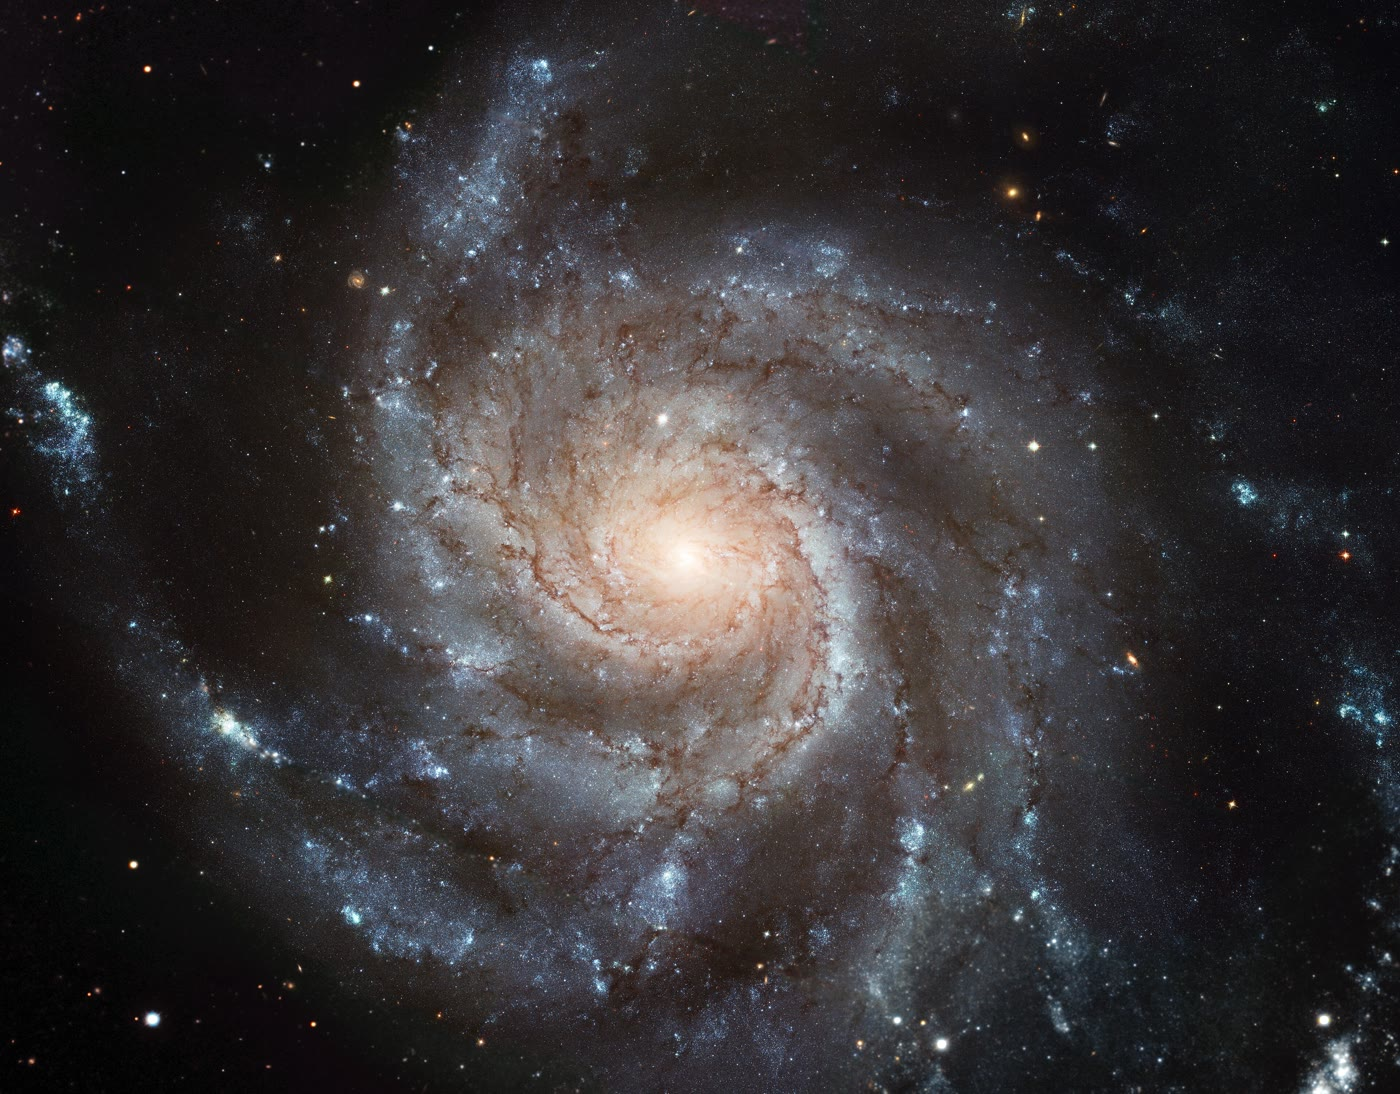
\includegraphics[width=0.66\linewidth]{images/book5/b3-m101.jpg}
\par\smallskip{\small \omterm{def:b3:milky-way-galaxies:types}{المجرّة الحلزونية} M101 مرئيّة من الأعلى بتلسكوب هابل
الفضائي، وهي فسيفساء من 51 تعريضًا، وقد قُصّت حوافها. انتفاخ صغير
ساطع يميل إلى الاصفرار؛ أذرع منفتحة أكثر زرقة ومعقودة بتجمّعات من النجوم الفتيّة؛
وشرائط بنّية من الغبار على طول الأذرع. الصورة: ESA وNASA
\mbox{\textdir TLT (Hubble, heic0602), CC BY~4.0}.}\label{fig:b3:milky-way-galaxies:m101}
\end{omfigure}
% ledger: photo:b3-m101

لماذا لا تلتفّ الأذرع \omterm{def:b3:milky-way-galaxies:types}{الحلزونية} على نفسها؟ في قرص يكون منحنى دورانه مسطّحًا،
تقطع نجمة تبعد نصف المسافة عن المركز الدورة في نصف الزمن.
فلو كانت الأذرع مؤلّفة من نجوم لالتفّت أكثر بإحكام مع كل دورة،
ولصارت بعد بضع دورات من القرص لفافة ضيّقة (انظر \cref{exo:b3:milky-way-galaxies:11}).

\begin{definition}[نظرية موجة الكثافة]\label{def:b3:milky-way-galaxies:density-wave}
تفسّر \emph{نظرية موجة الكثافة}\index{نظرية موجة الكثافة} الأذرع \omterm{def:b3:milky-way-galaxies:types}{الحلزونية}
بوصفها موجة من كثافة أعلى في القرص، نمطًا حلزونيًّا يدور
بصلابة بسرعته الزاوية الخاصّة، أي سرعة النمط، بينما تمرّ النجوم والغاز
عبره، فتتباطأ عند دخولها الذراع المزدحمة وتُسرع عند خروجها منها،
كما تمرّ السيارات عبر ازدحام مروري.
\end{definition}

اقترحت النظرية عام 1964، فحرّرت الأذرع من مشكلة الالتفاف.
يُضغط الغاز الداخل إلى الذراع، وتتكوّن فيه النجوم:
تُبرز الأذرعَ النجومُ الفتيّة والغازُ المتوهّج، فيما تنتشر النجوم المسنّة
توزيعًا أكثر انتظامًا بكثير. وما إذا كانت الأذرع موجات طويلة العمر فلا يزال محلّ جدل؛
فمحاكاة الأقراص الحاسوبية تُنتج في الغالب أذرعًا عابرة،
تتفكّك وتعاود التشكّل، ويمكن لمرور مجرّة أو لقضيب أن يُولِّد
حلزونًا ذا ذراعين.
% ledger: dobbs14:density-wave

\begin{definition}[الثقب الأسود الفائق الكتلة]\label{def:b3:milky-way-galaxies:smbh}
\emph{الثقب الأسود الفائق الكتلة}\index{الثقب الأسود الفائق الكتلة} هو ثقب أسود
كتلته مليون كتلة شمسية أو أكثر في مركز مجرّة.
\end{definition}

في مركز درب التبانة، يقع المصدر الراديوي المدمج الرامي~A*
(الرامي~A*) بين نجوم تدور في مدارات ضيّقة سريعة. تتطلّب مداراتها
كتلة مركزية تبلغ نحو أربعة ملايين شمس، $\num[separate-uncertainty=true]{4.2 \pm 0.2 e6}$
كتلة شمسية في مراجعة للقياسات. الرامي~A* بالكاد يتحرّك
بالنسبة إلى المجرّات البعيدة: بعد إزالة حركة الشمس المدارية، تكون حركته
الباقية لا تتجاوز بضعة كيلومترات في الثانية، فهو يحتفظ بما لا يقلّ
عن ربع تلك الكتلة. حجمه قابل للمقارنة مع شفارتزشيلد
نصف قطره، وكثافته التي تتجاوز \num{4e23} كتلة شمسية لكلّ
فرسخ فلكي مكعّب، قريبة جدًّا من تلك المتوقّعة لثقب أسود: والدليل
على أنّ الرامي~A* ثقب أسود ساحق.
% ledger: reid20:sgra, bhg16:structure, gravity19:r0

\begin{definition}[المجموعة المحلية؛ عنقود المجرّات]\label{def:b3:milky-way-galaxies:groups}
\emph{المجموعة المحلية}\index{المجموعة المحلية} هي المجموعة المترابطة بالجاذبية
من المجرّات، تهيمن عليها درب التبانة وأندروميدا، ولكلٍّ منهما
مجرّاته التابعة. \emph{عنقود المجرّات}\index{عنقود المجرّات} هو
أحد أكبر الأنظمة المترابطة بالجاذبية: مجرّات كثيرة محتجزة،
مع غاز ساخن يُشعّ الأشعّة السينية، في بئر جذبية مشتركة معظمها من المادة
المظلمة.
\end{definition}

يقع أكثر من مئة مجرّة ضمن \qty{3}{Mpc} من الشمس، معظمها
مجرّات قزمة. تبعد سحابة ماجلان الكبرى نحو \qty{50}{kpc}، وأندروميدا على
بُعد \qty{783}{kpc} وتقترب منّا بسرعة \qty{300}{km.s^{-1}}، وأعضاء المجموعة المرتبطة
تقع ضمن نحو \qty{1.06}{Mpc} من مركز كتلتها،
بين درب التبانة وأندروميدا، حيث تنأى عن
توسّع الكون. وتُستنتج كتلتها من حركة المجرّتين الكبيرتين
نحو بعضهما، فتبلغ من رتبة \num{5e12} كتلة شمسية. وفي
\omterm{def:b3:milky-way-galaxies:groups}{عنقود مجرّات} ضخم، يحتفظ الغاز الساخن عند نحو \qty{e8}{K}، بكتلة تبلغ نحو عشرة
أضعاف كتلة النجوم؛ والمجرّات والغاز معًا أخفّ من أن تفسّر عمق
البئر الجذبية، ومعظم كتلة العنقود،
من رتبة \num{e15} كتلة شمسية، فهي مظلمة.
% ledger: mcconn12:local-group, kravtsov12:clusters

\section{سلّم المسافات}\label{sec:b3:milky-way-galaxies:ladder}

يعطي الانزياح الظاهري مسافةً بالهندسة وحدها، لكنّ الانزياحات تتناقص مع
البُعد. أفضل كتالوج لها يقيس الانزياح الظاهري بعدم يقين
قدره 0.02 إلى \qty{0.03}{mas} للنجوم الأسطع من
القدر~15، فنحصل على مسافة دقيقة بنحو \qty{10}{\percent} حتى نحو
\qty{4}{kpc}؛ أمّا سحابة ماجلان الكبرى، على بُعد \qty{50}{kpc}، فيبلغ انزياحها الظاهري
\qty{0.02}{mas}. أمّا ما بعد ذلك، فتعتمد المسافات على أجرام تُعرف
إشعاعيتها.
% ledger: gaia:dr3, freedman19:trgb

\begin{definition}[الشمعة المعيارية؛ سلّم المسافات]\label{def:b3:milky-way-galaxies:ladder}
\emph{الشمعة المعيارية}\index{الشمعة المعيارية} هي فئة من الأجرام
تُعرف قدرها المطلق، أو يمكن استنتاجه من خاصّية تُقاس
بمعزل عن المسافة، بحيث يعطي قدرها الظاهر
معامل المسافة له. \emph{سلّم المسافات}\index{سلّم المسافات} هو
سلسلة من الطرائق، تُعاير كلٌّ منها على أجرام قريبة بما يكفي لتُقاس
أيضًا بالطريقة التي تسبقها، والتي تنقل المسافات من
الانزياحات الظاهرية حتى الكون المتمدّد.
\end{definition}

\begin{definition}[المتغيّر القيفاوي؛ قانون ليفيت]\label{def:b3:milky-way-galaxies:cepheid}
\emph{المتغيّر القيفاوي}\index{المتغيّر القيفاوي} هو نجم فتيّ، مشعّ،
نابض، يتغيّر سطوعه بدورة منتظمة تمامًا،
تتراوح من نحو يوم إلى عدّة أسابيع. أمّا \emph{قانون ليفيت}\index{قانون ليفيت}،
أو علاقة الدور--الإشعاعية، وهي العلاقة الخطّية بين متوسّط
القدر المطلق للمتغيّر القيفاوي ولوغاريتم دوره، فتكون الأدوار أطول
للنجوم الأسطع.
\end{definition}

اكتُشفت العلاقة في سحابة ماجلان الصغرى، التي تكون نجومها
جميعها على المسافة نفسها تقريبًا، وذلك عام 1908. الغبار في المجرّة التي
تحوي متغيّرًا قيفاويًّا يُخفته ويحمّره؛ لكنّ الإخماد يكون أكبر في
الضوء المرئي منه في تحت الحمراء القريبة، بنسبة ثابتة لنوع معيّن من
الغبار، ويُختار المزيج $W_I = I - 1.55\,(V - I)$ للأقدار في
النطاقين I وV، دليل ويسنهايت، بحيث
يُلغى الإخماد. يبيّن الشكل أدناه ذلك لعدد 2315 من المتغيّرات القيفاوية في
سحابة ماجلان الكبرى: \omterm{def:b3:milky-way-galaxies:cepheid}{قانون ليفيت} خطّ محكم، مع تشتّت قدره
\qty{0.078}{mag}، أي \qty{3.6}{\percent} في المسافة لنجم
واحد.
% ledger: sos15:leavitt, data:b5-ogle-lmc-cep

\begin{omfigure}
\centering
\begin{tikzpicture}
\begin{axis}[width=0.80\linewidth, height=0.52\linewidth,
  xmin=-0.05, xmax=1.6, ymin=10, ymax=16.6, y dir=reverse,
  xlabel={$\log_{10}(P/\mathrm{d})$}, ylabel={دليل ويسنهايت $W_I$ \babelsublr{(\unit{mag})}},
  tick label style={font=\scriptsize}, label style={font=\small},
  legend style={font=\scriptsize, at={(0.5,-0.17)}, anchor=north, legend columns=3, draw=none, cells={anchor=west}, /tikz/every even column/.append style={column sep=1em}},
  legend image post style={scale=2.2}]
\addplot[only marks, mark=*, mark size=0.45pt, omDef, opacity=0.6] table[x=logp, y=w] {figdata/out/bachelor-3-distance_ladder-pl.dat};
\addlegendentry{المتغيّرات القيفاوية}
\addplot[only marks, mark=x, mark size=1.6pt, red!70!black] table[x=logp, y=w] {figdata/out/bachelor-3-distance_ladder-clipped.dat};
\addlegendentry{\foreignlanguage{arabic}{المستبعدة ($>3\sigma$)}}
\addplot[thick, black] table[x=logp, y=w_fit] {figdata/out/bachelor-3-distance_ladder-fit.dat};
\addlegendentry{الملاءمة}
\node[font=\scriptsize, anchor=south west, fill=white, inner sep=1pt] at (axis cs:0.55,11.0) {$W_I = -3.315\log_{10}P + 15.889$};
\end{axis}
\end{tikzpicture}
\par\smallskip{\small \omterm{def:b3:milky-way-galaxies:cepheid}{قانون ليفيت} في سحابة ماجلان الكبرى:
دليل ويسنهايت لعدد 2315 من المتغيّرات القيفاوية النابضة بنمطها الأساسي
مقابل لوغاريتم أدوارها (مسح \babelsublr{OGLE}، سوشينسكي وآخرون،
2015، عبر \babelsublr{CDS}). النجوم الأسطع تقع أعلى. خطّ مستقيم
مُلائم بطريقة المربعات الصغرى، بعد استبعاد 92 نجمًا تبعد أكثر من ثلاثة
انحرافات معيارية عنه، يعيد إنتاج العلاقة المنشورة
($-3.314$، $15.888$). ومع معامل المسافة للسحابة، 18.477، يعطي الخطّ
يعطي قدر ويسنهايت المطلق لأيّ متغيّر قيفاوي انطلاقًا من دوره.}\label{fig:b3:milky-way-galaxies:leavitt}
\end{omfigure}
% ledger: data:b5-ogle-lmc-cep, sos15:leavitt, freedman19:trgb

\begin{definition}[قمّة فرع العمالقة الحمراء]\label{def:b3:milky-way-galaxies:trgb}
\emph{قمّة فرع العمالقة الحمراء}\index{قمّة فرع العمالقة الحمراء}
(TRGB) هي الحدّ الأعلى الحادّ لإشعاعيات العمالقة الحمراء في
لجمهرة نجمية قديمة، يحدّده إشعال الهيليوم في لُبّ نجومها،
الوميض الهيليومي؛ وفي نطاق I يقع القدر المطلق تقريبًا عند القيمة نفسها
في كلّ جمهرة قديمة، عند قدر $M_I \approx -4.05$ وعند لون
$V - I = 1.6$، ويعتمد اعتمادًا ضعيفًا فقط على التركيب الكيميائي.
\end{definition}

تُقاس القمّة في الهالات المتناثرة للمجرّات، حيث
قليل الغبار وقليل الازدحام؛ فهي تستعمل نجومًا هالية قديمة، حيث تستعمل القيفاويات
نجومًا قرصية فتية، ولا تشترك الطريقتان في أيّ مبدأ فيزيائي. تبلغ القيفاويات
وTRGB بضع عشرات من الميغابارسك، وتصل إلى مجرّات انفجرت فيها شمعة معيارية نادرة
وأشدّ سطوعًا بكثير: المستعر الأعظم من النوع \babelsublr{Ia}، وهو
الانفجار النووي الحراري لقزم أبيض، كما ورد في كتب الفيزياء،
الذي يبلغ قدره المطلق الذروي، بعد تصحيحه من أجل
شكل منحنى ضوئه ولونه، هو
$M_B = \qty[separate-uncertainty=true]{-19.253 \pm 0.027}{mag}$. وتُرصد هذه
المستعرات عبر مئات الميغابارسكات.
% ledger: freedman19:trgb, riess22:h0

\begin{definition}[علاقة تولي--فيشر]\label{def:b3:milky-way-galaxies:tully-fisher}
\emph{علاقة تولي--فيشر}\index{علاقة تولي--فيشر} هي
الترابط بين الإشعاعية، أو بالأحرى كتلة النجوم والغاز،
لمجرّة حلزونية وسرعة منحنى دورانها المسطّح؛ وفي صيغته
الباريونية $M_\mathrm{b} = A\,V^4$، فإنّه يصحّ من نحو 30 إلى
\qty{300}{km.s^{-1}}.
\end{definition}

يعطي طيف 21 سم لمجرّة ما أقصى سرعة دورانها، وتعطي العلاقة
إشعاعيتها مستقلّةً عن بُعدها، ثم يعطي فيضُها البُعدَ:
مرتبةٌ للمجرّات \omterm{def:b3:milky-way-galaxies:types}{الحلزونية} البعيدة أكثر مما تبلغه
النجوم المفردة. ويقع درب التبانة، بإشعاعيته ودورانه، على العلاقة.
% ledger: mcgaugh00:btf, nrao:hi-line, bhg16:structure

\begin{omfigure}
\centering
\pgfplotstableread{figdata/out/bachelor-3-distance_ladder-ladder.dat}\laddertab
\pgfplotstableread{figdata/out/bachelor-3-distance_ladder-anchors.dat}\anchortab
\pgfplotstablegetelem{0}{d_hi}\of{\laddertab}\let\plxhi\pgfplotsretval
\pgfplotstablegetelem{1}{d_lo}\of{\laddertab}\let\cephlo\pgfplotsretval
\pgfplotstablegetelem{1}{d_hi}\of{\laddertab}\let\cephhi\pgfplotsretval
\pgfplotstablegetelem{3}{d_lo}\of{\laddertab}\let\snlo\pgfplotsretval
\pgfplotstablegetelem{3}{d_hi}\of{\laddertab}\let\snhi\pgfplotsretval
\pgfplotstablegetelem{1}{d}\of{\anchortab}\let\mthirtyone\pgfplotsretval
\pgfplotstablegetelem{2}{d}\of{\anchortab}\let\nfourtwo\pgfplotsretval
\begin{tikzpicture}
\begin{axis}[width=0.92\linewidth, height=0.42\linewidth,
  xmode=log, xmin=1e-3, xmax=2e6, ymin=0.4, ymax=4.9,
  ytick={1,2,3,4}, yticklabels={التزيّح المنظوري, القيفاويات, TRGB, \babelsublr{SNe~Ia}},
  xtick={1e-3,1e-2,1e-1,1,10,100,1e3,1e4,1e5,1e6},
  xticklabels={1~pc,,,1~kpc,,,1~Mpc,,,1~Gpc},
  xlabel={المسافة}, tick label style={font=\scriptsize}, label style={font=\small},
  y tick label style={font=\small}, axis y line*=left, axis x line*=bottom]
\draw[line width=7pt, omDef!70] (axis cs:1e-3,1) -- (axis cs:\plxhi,1);
\draw[line width=7pt, omMeth!70] (axis cs:\cephlo,2) -- (axis cs:\cephhi,2);
\draw[line width=7pt, omProp!70] (axis cs:\cephlo,3) -- (axis cs:\cephhi,3);
\draw[line width=7pt, red!60] (axis cs:\snlo,4) -- (axis cs:\snhi,4);
\draw[densely dotted, thick] (axis cs:\cephlo,0.4) -- (axis cs:\cephlo,4.55) node[anchor=south, font=\scriptsize] {LMC};
\draw[densely dotted, thick] (axis cs:\mthirtyone,0.4) -- (axis cs:\mthirtyone,4.55) node[anchor=south, font=\scriptsize] {M31};
\draw[densely dotted, thick] (axis cs:\nfourtwo,0.4) -- (axis cs:\nfourtwo,4.55) node[anchor=south, font=\scriptsize] {NGC~4258};
\draw[->, thick, black!60] (axis cs:\plxhi,1.25) to[out=30, in=200] (axis cs:\cephlo,1.75);
\draw[->, thick, black!60] (axis cs:\cephhi,2.25) to[out=40, in=220] (axis cs:\snlo,3.75);
\end{axis}
\end{tikzpicture}
\par\smallskip{\small مراتب \omterm{def:b3:milky-way-galaxies:ladder}{سلّم المسافات}، مع المدى الذي تُستعمل فيه كلّ مرتبة هنا:
عمليات قياس التزيّح المنظوري لأفضل كتالوج، حتى \qty{10}{\percent} حتى
\qty{4}{kpc}؛ القيفاويات وفرع العمالقة الحمراء من سحابة ماجلان الكبرى حتى
مضيفات أقرب المستعرات الأعظم من النوع \babelsublr{Ia}، \qty{45}{Mpc}؛
المستعرات الأعظم للتمدّد المنتظم، عند إزاحات حمراء من 0.023 إلى 0.15
(\qtyrange{96}{616}{Mpc} من أجل $H_0 = 73$). المنقّطة: مرساتان لمقياس
القيفاويات بمسافات هندسية (الثنائيات الكاسفة في سحابة ماجلان الكبرى،
والمازرات المائية التي تدور حول الثقب الأسود في \babelsublr{NGC~4258})،
و\babelsublr{M31}، أقرب حلزونية كبيرة. الأسهم: تُعايَر كلّ مرتبة على أجرام
تقيسها أيضًا المرتبة الواقعة تحتها، فالقيفاويات في المجرّة بتزيّحاتها
المنظورية، والمستعرات الأعظم في المجرّات القريبة بالقيفاويات وفرع العمالقة
الحمراء في مضيفاتها.}\label{fig:b3:milky-way-galaxies:ladder-rungs}
\end{omfigure}
% ledger: gaia:dr3, riess22:h0, freedman19:trgb, mcconn12:local-group

في أعلى السلّم، تقيس المستعرات الأعظم تمدّد
الكون. ينصّ قانون هابل، كما ورد في كتب الفيزياء، على أنّ سرعة
التباعد $cz$ لمجرّة بعيدة تتناسب طرديًّا مع بُعدها $d$،
$cz = H_0 d$ عند إزاحات حمراء صغيرة $z$؛ وثابت هابل $H_0$ هو
الميل، والمستعرات الأعظم، مع مسافاتها المأخوذة من السلّم، تعطيه.

\begin{definition}[توتّر هابل]\label{def:b3:milky-way-galaxies:tension}
\emph{توتّر هابل}\index{توتّر هابل} هو الخلاف
بين قيمة ثابت هابل المقاسة محلّيًّا \omterm{def:b3:milky-way-galaxies:ladder}{بسلّم المسافات}،
والقيمة المستنتجة من خلفية الموجات الدقيقة الكونية
بالنموذج الكوني المعياري.
\end{definition}

\begin{dated}{2022}
القيفاويات في مضيفات 42 مستعرًا أعظم من النوع \babelsublr{Ia}، مرساةً على تزيّحات غايا المنظورية،
والمازرات \babelsublr{NGC~4258} والثنائيات الكاسفة في
سحابة ماجلان الكبرى، تعطي
$H_0 = \qty[separate-uncertainty=true]{73.04 \pm 1.04}{km.s^{-1}.Mpc^{-1}}$.
وأعطت \omterm{def:b3:milky-way-galaxies:trgb}{قمّة فرع العمالقة الحمراء}، بمعايرة نحو مائة مستعر أعظم،
في عام 2019 $H_0 = 69.8 \pm 0.8 \pm \qty{1.7}{km.s^{-1}.Mpc^{-1}}$
(إحصائي ومنهجي). وخريطة القمر الصناعي بلانك للخلفية
الكونية للموجات الدقيقة، وإذا قُرئت بالنموذج الكوني المعياري، تُفضي إلى
$H_0 = \qty[separate-uncertainty=true]{67.4 \pm 0.5}{km.s^{-1}.Mpc^{-1}}$.
وتختلف قيمة القيفاويات عن قيمة الخلفية بمقدار خمسة انحرافات
معيارية؛ وتقع قيمة TRGB بينهما. ومصدر
التناقض غير معروف: خطأ لم يُكتشف بعدُ في أحد السلّمين،
أو فيزياء ناقصة في النموذج.
\end{dated}
% ledger: riess22:h0, freedman19:trgb, planck18:h0

\begin{inthelab}[ساتل قياس المواقع الفلكية وكتالوجه]
يمسح الساتل غايا السماءَ وفق نمطٍ مُبرمَج، بحيث تُقاس كلُّ
نجمٍ مرارًا وتكرارًا خلال المهمّة. وعلى الأرض، تحوّل وحدات التنسيق في
كونسورتيوم معالجة البيانات هذه القياسات إلى موضعٍ وانزياحٍ منظوريٍّ وحركةٍ ذاتيةٍ لكلّ
مصدرٍ من أكثر من مليار مصدر: فمن الحركات الصغيرة لنجمٍ على السماء،
يكون الانزياح المنظوري هو الجزء الذي يتكرّر كلّ عام،
والحركة الذاتية هي الجزء الذي يتراكم. وتُنشر كلّ قائمة مع أوراقٍ
تصف معالجتها وتحقّقها، وكلّ مسافة في أشكال هذا القسم
التي تعتمد على انزياحٍ منظوريٍّ
تعتمد في النهاية على
كتالوج من هذا النوع.
\end{inthelab}

\begin{dated}{2022}
الكتالوج الثالث للساتل غايا، الصادر في 13 يونيو 2022 من 34 شهرًا من
الرصد، يعطي المواضع والانزياحات المنظورية والحركات الذاتية لنحو
1.46~مليار مصدر، من القدر~3 إلى~21، ومتوسّطات السرعة الشعاعية
33~مليون نجم. وتبلغ شكوك الانزياح المنظوري 0.02 إلى
\qty{0.03}{mas} للنجوم الأسطع من القدر~15، و\qty{0.07}{mas} عند
القدر~17، و\qty{0.5}{mas} عند القدر~20.
\end{dated}
% ledger: gaia:dr3

\section{التمارين}

\begin{exercise}[$\star$]\label{exo:b3:milky-way-galaxies:1}
سنة الشمس المجرّية. (أ)~بأخذ $R_0 = \qty{8.178}{kpc}$
و$V_0 = \qty{229}{km.s^{-1}}$، احسب دور مدار الشمس حول
مركز المجرّة، بالملايين من السنين. (ب)~كم مرّةً دارت الشمس
منذ تشكّل المجموعة الشمسية، قبل \qty{4.54}{Gyr}؟
\end{exercise}

\begin{exercise}[$\star$]\label{exo:b3:milky-way-galaxies:2}
الحركة الارتدادية للمصدر الرامي~A*. (أ)~حركة ذاتية مقدارها \qty{1}{mas} في السنة
عند \qty{1}{kpc} تكافئ سرعة مستعرضة قدرها \qty{1}{au} في السنة: عبّرْ عنها
بالكيلومترات في الثانية. (ب)~المصدر الرامي~A*، مفترَضًا ساكنًا عند مركز المجرّة
عند \qty{8.178}{kpc}، ينجرف على طول المستوى المجرّي بمقدار \qty{6.411}{mas}
في السنة. احسب سرعة الشمس حول المركز، وقارنها بالقيمة
المرجعية، \qty[separate-uncertainty=true]{248 \pm 3}{km.s^{-1}}. (ج)~اطرح الحركة
الخاصة للشمس في اتجاه الدوران، \qty{11}{km.s^{-1}}، ثم قارن النتيجة
بالقيمة $V_0$ المستخرجة من \omterm{def:b3:milky-way-galaxies:rotation-curve}{منحنى الدوران}.
\end{exercise}

\begin{exercise}[$\star$]\label{exo:b3:milky-way-galaxies:3}
تصنيف المجرّات \omterm{def:b3:milky-way-galaxies:types}{الإهليلجية}. (أ)~لخطوط التساوي الضوئي في مجرّة إهليلجية
نسبةُ محورين قدرها 0.6: حدّد صنفها. (ب)~ما نسبة المحورين لمجرّة E7؟
(ج)~لماذا قد تكون المجرّة E0 نظامًا مفلطحًا؟
\end{exercise}

\begin{exercise}[$\star$]\label{exo:b3:milky-way-galaxies:4}
نقاط الارتكاز. احسب مسافات سحابة ماجلان الكبرى
($\mu = 18.477$)، وأندروميدا ($\mu = 24.47$) و\mbox{\textdir TLT NGC~4258}
($\mu = 29.398$). ما الانزياح المنظوري الذي يكون لنجمٍ في السحابة، ولماذا
لا يمكن قياس مسافة السحابة بالانزياحات المنظورية؟
\end{exercise}

\begin{exercise}[$\star\star$]\label{exo:b3:milky-way-galaxies:5}
انطلاقًا من ثابتي أورت $A = \qty{15.3}{km.s^{-1}.kpc^{-1}}$
و$B = \qty{-11.9}{km.s^{-1}.kpc^{-1}}$: (أ)~احسب السرعة الزاوية
\omterm{def:b3:milky-way-galaxies:lsr}{لمعيار السكون المحلي} LSR، ثم، بأخذ $R_0 = \qty{8.178}{kpc}$، السرعة الدائرية $V_0$؛
(ب)~احسب ميل \omterm{def:b3:milky-way-galaxies:rotation-curve}{منحنى الدوران} عند الشمس. (ج)~قارن
بمنحنى دوران العمالقة الحمراء ($V_0 = \qty{229.0}{km.s^{-1}}$،
ميله \qty{-1.7}{km.s^{-1}} لكلّ كيلوفرسخ)، واقترح سببَ اختلاف المنحنيين،
علمًا بأنّ القياس نفسه وجد $C$ و$K$ غيرَ صفريّين.
\end{exercise}

\begin{exercise}[$\star\star$]\label{exo:b3:milky-way-galaxies:6}
الكثافة المحلية \omterm{def:b3:milky-way-galaxies:rotation-curve}{ومنحنى الدوران} المستوي. (أ)~لمجرّة كروية
ذات منحنى دوران مستوٍ عند \qty{229}{km.s^{-1}}، احسب الكثافة عند
\qty{8.178}{kpc}، بوحدة الكتل الشمسية لكلّ فرسخ فلكي مكعّب
($G = \qty{4.301e-6}{kpc.(km.s^{-1})^2}$ لكلّ كتلة شمسية). (ب)~بيّن أنّ
كتلة شمسية واحدة لكلّ فرسخ فلكي مكعّب تساوي \qty{37.96}{GeV.cm^{-3}}، وعبّر
عن كثافة المادة المظلمة المحلية، \qty{0.30}{GeV.cm^{-3}}، بوحدة الكتل الشمسية
لكلّ فرسخ فلكي مكعّب. (ج)~لماذا تكون الكثافة في (أ) أكبر؟
\end{exercise}

\begin{exercise}[$\star\star$]\label{exo:b3:milky-way-galaxies:7}
مسافة متغيّر قيفاوي. في مجرّة حلزونية متخيَّلة، لدينا متغيّر قيفاوي دوره
\qty{30}{d}، ومتوسط دليل فيسنهايت $W_I = \qty{25.00}{mag}$.
(أ)~باستخدام \omterm{def:b3:milky-way-galaxies:cepheid}{قانون ليفيت} لسحابة ماجلان الكبرى،
$W_I = -3.314\log_{10}P + 15.888$، ومعامل المسافة للسحابة
18.477، احسب القدر المطلق لفيسنهايت للمتغيّر القيفاوي. (ب)~احسب
مسافة المجرّة. (ج)~يبلغ تشتّت القانون \qty{0.077}{mag}: ما
الخطأ النسبي في المسافة من متغيّر قيفاوي واحد، ومن خمسين؟
\end{exercise}

\begin{exercise}[$\star\star$]\label{exo:b3:milky-way-galaxies:8}
مسافة TRGB. في هالة مجرّة متخيَّلة، تقع \omterm{def:b3:milky-way-galaxies:trgb}{قمّة فرع
العمالقة الحمراء} عند $I = \qty{26.00}{mag}$؛ ويُخفّت الغبار على امتداد خط
النظر نطاقَ I بمقدار \qty{0.05}{mag}. بفرض $M_I = -4.05$، احسب
معامل المسافة والمسافة. ماذا يعني عدم اليقين البالغ
\qty{0.04}{mag} في القمّة بالنسبة إلى المسافة؟
\end{exercise}

\begin{exercise}[$\star\star$]\label{exo:b3:milky-way-galaxies:9}
ثابت هابل من المستعرات العظمى. لمستعر أعظم في
التمدّد المنتظم، $\log_{10}(cz) - 0.2\,m_B = a_B$، وهو مقطع
مخطط هابل للمستعرات العظمى، ومعامل المسافة هو
$m_B - M_B = 5\log_{10}(d/\mathrm{Mpc}) + 25$. (أ)~بيّن أنّ
$\log_{10}H_0 = 0.2\,M_B + a_B + 5$ ($H_0$ بالكيلومترات في الثانية لكلّ
ميغافرسخ). (ب)~بأخذ $M_B = -19.253$ و$a_B = 0.714158$، احسب $H_0$.
(ج)~ما $M_B$ الذي يعطي $H_0 = \qty{67.4}{km.s^{-1}.Mpc^{-1}}$؟ بكم
قدرًا، وبأيّ كسرٍ من المسافات، تختلف
المعايرتان؟
\end{exercise}

\begin{exercise}[$\star\star\star$]\label{exo:b3:milky-way-galaxies:10}
من أين تأتي \omterm{def:b3:milky-way-galaxies:tully-fisher}{علاقة تولي--فيشر}. (أ)~لمجرّة قرصية كتلتها $M$
ونصف قطرها $R$ تدور بسرعة $V$: بيّن أنّ $M \approx RV^2/G$. (ب)~إذا كانت جميع
المجرّات \omterm{def:b3:milky-way-galaxies:types}{الحلزونية} تملك متوسط كثافة السطح نفسها $\Sigma = M/(\pi R^2)$،
بيّن أنّ $M \propto V^4$. (ج)~مجرّتان متخيَّلتان على العلاقة الباريونية نفسها
تدوران بسرعة 100 و\qty{229}{km.s^{-1}}: ما نسبة
كتلتيهما؟ (د)~تدور مجرّتان بالسرعة نفسها، ولهما
الإشعاعية نفسها؛ وتعطي إحداهما أربعة أمثال دفق الأخرى. قارن
بين مسافتيهما.
\end{exercise}

\begin{exercise}[$\star\star\star$]\label{exo:b3:milky-way-galaxies:11}
مسألة الالتفاف. يدور قرص بمنحنى دوران مستوٍ عند
\qty{229}{km.s^{-1}}. (أ)~حوّل هذه السرعة إلى كيلوفرسخ فلكي لكل مليار
سنة. (ب)~ذراعٌ مستقيم من النجوم يمتدّ عند الزمن صفر من 4 إلى
\qty{12}{kpc}. احسب دورَي المدار عند طرفيه. (ج)~بعد
\qty{1}{Gyr}، بأيّ زاوية تقدّم طرفه الداخلي على طرفه
الخارجي؟ كم لفّة حلزونية يمثّل ذلك، وكيف يبدو
الذراع؟ (د)~كيف تتجنّب موجة الكثافة ذلك؟
\end{exercise}

\begin{exercise}[$\star\star\star$]\label{exo:b3:milky-way-galaxies:12}
الثقب الأسود في المركز. لتكن الكتلة المركزية
\num{4.2e6} كتلة شمسية و$R_0 = \qty{8178}{pc}$. (أ)~النجم S2
يدور حوله في \num{16}~سنة: احسب نصف المحور الأكبر لمداره بالوحدة
الفلكية (قانون كبلر الثالث بالوحدات الشمسية، $a^3 = MP^2$ مع
$a$ بالوحدة الفلكية، $P$ بالسنوات و$M$ بالكتل الشمسية)، والحجم الزاوي لمداره كما يُرى
من الأرض. (ب)~احسب نصف قطر شفارتزشيلد للثقب الأسود بالأمتار
وبالوحدات الفلكية، والزاوية التي يحصرها قطره
من الأرض، بالميكروثانية القوسية. (ج)~احسب متوسط كثافة
الكتلة داخل نصف قطر شفارتزشيلد، بالكتل الشمسية لكل
فرسخ فلكي مكعّب، وقارنها بالحدّ الأدنى الذي تفرضه حركة الرامي~A*،
\num{4e23} كتلة شمسية لكل فرسخ فلكي مكعّب.
\end{exercise}

\section{مسألة: وزن المجرّة}

\begin{problem}[{مسألة نهاية الأسبوع --- من حركات النجوم والغاز إلى
المادة المظلمة داخل \qty{20}{kpc}}]
\label{pb:b3:milky-way-galaxies:1}
لتكن $R_0 = \qty{8.18}{kpc}$، و$G = \qty{4.301e-6}{kpc.(km.s^{-1})^2}$ لكل
كتلة شمسية، و\qty{4.74}{km.s^{-1}} للحركة الذاتية البالغة
\qty{1}{mas} سنويًا عند \qty{1}{kpc}. تُقاس جميع السرعات بالنسبة إلى
LSR. استعمل مبرهنتَي أورت ومبرهنة النقطة المماسّية في الفصل، والتقريب
الكروي $M = RV^2/G$ للكتل الديناميكية.

\medskip\noindent\textbf{الجزء الأول --- الدوران المحلي.} مسحٌ مُتخيَّل
لنجوم التجمّع الأحمر، جميعها عند $d = \qty{1.00}{kpc}$ في المستوي
المجرّي، يعطي متوسط السرعة الشعاعية \qty{+15.4}{km.s^{-1}} عند
$\ell = \ang{45}$ و\qty{-15.2}{km.s^{-1}} عند $\ell = \ang{135}$،
ومتوسط الحركات الذاتية في خط الطول \qty{-5.91}{mas} سنويًا عند
$\ell = \ang{90}$ و\qty{+0.55}{mas} سنويًا عند $\ell = \ang{0}$.
\begin{enumerate}
\item ماذا تتنبّأ صيغة أورت للسرعات الشعاعية عند
  $\ell = \ang{45}$، \ang{90}، \ang{135} و\ang{180}؟
\item احسب $A$ من السرعتين الشعاعيتين.
\item احسب $B$ من الحركة الذاتية عند $\ell = \ang{90}$.
\item احسب $B$ مرّةً أخرى من الحركة الذاتية عند $\ell = \ang{0}$،
  وقارِن النتيجتين.
\item احسب السرعة الزاوية \omterm{def:b3:milky-way-galaxies:lsr}{لمعيار السكون المحلي} LSR والسرعة الدائرية
  $V_0$.
\item احسب ميل \omterm{def:b3:milky-way-galaxies:rotation-curve}{منحنى الدوران} عند الشمس. هل المنحنى
  صاعد أم مستوٍ أم هابط؟
\item احسب دور مدار الشمس وعدد الدورات التي تتمّها
  خلال \qty{4.54}{Gyr}.
\end{enumerate}

\medskip\noindent\textbf{الجزء الثاني --- \omterm{def:b3:milky-way-galaxies:rotation-curve}{منحنى الدوران} الداخلي.} لتكن
$V_0 = \qty{229}{km.s^{-1}}$. أعلى السرعات الشعاعية في
ملامح \mbox{\textdir TLT 21-cm} عند $\ell = \ang{40}$، \ang{50}، \ang{60} و\ang{70} هي
82.9، 55.6، 32.4 و\qty{14.9}{km.s^{-1}}.
\begin{enumerate}[resume]
\item لماذا تحتاج طريقة النقطة المماسّية إلى $\ang{0} < \ell < \ang{90}$
  (أو الربع المرآتي)، ولماذا تفشل خارج الدائرة الشمسية؟
\item احسب نصف قطر النقطة المماسّية لكل خط طول.
\item احسب $V(R)$ عند كل نقطة مماسّية.
\item بكم، بالكيلوهرتز، يُزاح خط الغاز عند النقطة المماسّية
  عند $\ell = \ang{40}$ عن تردّده السكوني،
  \qty{1420.405751}{MHz}، وفي أيّ اتجاه؟
\item قارِن بمنحنى العمالقة الحمراء، الذي يعطي \qty{226.8}{km.s^{-1}}
  عند \qty{5.27}{kpc} و\qty{229.6}{km.s^{-1}} عند \qty{7.22}{kpc}. هل
  المنحنى الداخلي صاعد أم مستوٍ أم هابط؟
\item لو كانت السرعة عند النقطة المماسّية عند $\ell = \ang{40}$ هي سرعة
  كتلة نقطية في المركز تحمل الشمس بالسرعة $V_0$، فكم تكون؟
  ماذا تقول المقارنة عن توزيع الكتلة؟
\end{enumerate}

\medskip\noindent\textbf{الجزء الثالث --- الكتلة المرئية.} استعمل نموذج الكتلة
في الفصل، بوحدات الكتل الشمسية والكيلوفرسخ الفلكي: انتفاخ
بلامر $M = \num{1.067e10}$، $b = 0.3$؛ قرص رقيق من نوع مياموتو--ناغاي
$M = \num{3.944e10}$، $a = 5.3$، $b = 0.25$؛ وقرص سميك من الكتلة نفسها
مع $a = 2.6$، $b = 0.8$.
\begin{enumerate}[resume]
\item احسب الكتلة المرئية الكلّية للنموذج، وقارنها بالقيمة
  المرجعية لكتلة المجرّة النجمية، \qty[separate-uncertainty=true]{5 \pm 1 e10}{} كتل
  شمسية.
\item احسب السرعة الدائرية للانتفاخ وحده عند \qty{20}{kpc}.
\item احسب السرعتين الدائريتين للقرص الرقيق \omterm{def:b3:milky-way-galaxies:structure}{والقرص السميك} عند \qty{20}{kpc}.
\item احسب السرعة الدائرية لكل الكتلة المرئية عند
  \qty{20}{kpc}.
\item احسب القيمة نفسها عند $R_0$، وقارنها بالسرعة $V_0$.
\item لو تركّزت الكتلة المرئية كلّها في المركز، فما
  السرعة عند \qty{20}{kpc}؟ لماذا تقترب قيمة النموذج منها؟
\end{enumerate}

\medskip\noindent\textbf{الجزء الرابع --- المادة المظلمة.} العمالقة الحمراء
تعطي سرعة دائرية قدرها \qty{200}{km.s^{-1}} عند \qty{20}{kpc}.
\begin{enumerate}[resume]
\item احسب الكتلة الديناميكية داخل \qty{20}{kpc}.
\item احسب الكتلة الديناميكية للمادة المرئية داخل
  \qty{20}{kpc}.
\item احسب كتلة المادة المظلمة داخل \qty{20}{kpc}، وبيّن أنّ
  نسبتها هي $1 - (V_\mathrm{vis}/V)^2$.
\item الهالة NFW المُطابَقة على المنحنى كلّه تملك
  $\rho_0 = \num{1.06e7}$ كتلة شمسية لكل كيلوفرسخ فلكي مكعّب،
  و$R_s = \qty{14.8}{kpc}$. احسب كتلتها داخل \qty{20}{kpc}
  والنسبة المظلمة التي تُنتجها. لماذا تختلف عن الإجابة السابقة؟
\item احسب كثافة تلك الهالة عند $R_0$، بالكتل الشمسية لكل
  فرسخ فلكي مكعّب، وبالوحدة \unit{GeV.cm^{-3}} (كتلة شمسية واحدة لكل فرسخ فلكي مكعّب
  تساوي \qty{37.96}{GeV.cm^{-3}}).
\item أعطِ نسبة المادة المظلمة من الكتلة داخل \qty{20}{kpc}
  المستخلصة من السرعة المقيسة، بالنسبة المئوية، إلى رقمين
  معنويين.
\end{enumerate}
\end{problem}
% ledger: gravity19:r0, eilers19:table1, pouliasis17:model1, eilers19:halo, bhg16:structure, nrao:hi-line, const:G, const:au, iau:parsec, usgs:age-earth
